
\documentclass[11pt,a4paper]{article}
\usepackage{amsmath}
\usepackage{amsfonts}
\usepackage{graphics}
\usepackage{color}
\usepackage{tikz}
\usepackage{hyperref}
\usepackage{subfig} 

\title{\bf Optimisation tricks for \textit{Moments}} 

\begin{document}

\maketitle

This document gathers several ways of optimization for \textit{Moments} we thought about. 
It is probably not exhaustive but mentions the most important tricks we tried. Some of these tricks have been introduced in the software, other not. For each, we try to explain the global idea and if we decided not to include it in the \textit{Moments} for the 'moment' we explain why. 

\section{Cythonization}
Large matrices are needed to construct the linear system we solve in \textit{Moments}, be it the selection, drift or migration matrices or the Jackknife interpolators. This prior step could be an important part of the computation time with the naive python code. As these functions are mainly composed of loops and simple operations, we decided to code them in \href{http://cython.org}{\color{blue}\underline{Cython}}, a C extension of Python. Doing that led to a consequent speed up for the initialization step.\\

We use a tridiagonal solver (see next sections) for some very specific cases (neutral without migrations). For this specific configuration, we decided not to use python solvers and to code our own one. As it is mainly composed, here again, of loops and basic operations that are called a large amount of times, we also "cythonized" this part of the code gaining approximately a factor 2 on the tridiagonal system resolution.\\

We didn't "cythonize" very deeply, mainly specifying variable types. It is possible that other adjustments can improve a bit more the performances...

\section{Choice of the linear solvers and system pre-conditionning}
Whatever the case, most of the computation time is spent in the linear system solver. Consequently the choice of an appropriate solver is crucial. \\
Our linear system is banded and sparse. We can take advantage of it to save computation time as well as memory (we don't want to store all the 0s!) using a sparse solver that exploits this specificity. Scipy Python library contains specific classes and methods for sparse systems: \href{http://docs.scipy.org/doc/scipy/reference/sparse.html}{\color{blue}\underline{Scipy.sparse}}. We use the \href{http://docs.scipy.org/doc/scipy/reference/generated/scipy.sparse.coo_matrix.html#scipy.sparse.coo_matrix}{\color{blue}\underline{coo\_matrix}} format to build the matrices we need to solve the system. Then we use the \href{http://docs.scipy.org/doc/scipy/reference/sparse.linalg.html#module-scipy.sparse.linalg}{\color{blue}\underline{linalg}} sub package to inverse the system at each time step. We use a 2 steps method, first we pre-factorize the evolution matrix (\href{http://docs.scipy.org/doc/scipy/reference/generated/scipy.sparse.linalg.factorized.html#scipy.sparse.linalg.factorized}{\color{blue}\underline{factorized}}) and then we solve the system using the pre-factorization.
The main advantage of this 2-steps method is that the first step is only necessary when the evolution matrix has change since the last time step (typically when the population sizes change). 
This is the most efficient approach among those we tested: the naive numpy solver as well as a multiband solver. 

In some very special cases (neutral without selection) we use a homemade tridiagonal solver, faster than the sparse one.

\section{Dimension splitting}
	One of the main aims of this project was to take advantage of the new formulation to simulate more complex models than $\partial a \partial i$ can handle. The naive way to handle the resolution of a multidimensional linear system is to reshape the multi-d AFS into a vector. In that case the matrix of the linear system we need to inverse every time step is $n_s^d \times n_s^d$, where $n_s$ is the sample size (we assume the same for each population) and $d$ is the dimension of the problem (number of populations). This approach works but the scalability in terms of sample size as well as number of dimensions is really bad! For more than 3 populations, simulations are very slow even with the sparse solver and thus we are not that more efficient than $\partial a \partial i$.\\
	
	A rather common trick when dealing with multi dimensional PDEs (for instance diffusion equations) is to directionally split the operators. Even $\partial a \partial i$ uses this splitting. It consists in subdividing the multi-d resolution into several lower dimension (generally 1D) problems integrating alternately along the different axes. For instance, in a 2D case, if your operators can be splitted along each axis, instead of solving a big $n^2 \times n^2$ system, you solve a $n \times n$ system for each sub-vector of your 2D field, \textit{i.e.} $2n$ $n \times n$ systems. As the complexity of system inversion grows generally fast (depends on the solver you use) with the size of the system this splitting approach saves generally a lot of time.\\ 
	
	In our case things are a bit more complicated... Because of migration terms, we have to deal with "crossed terms" of the form $\Phi_n(i_1+1, i_2-1)$ making it impossible to use a conventional uni-directional splitting (contrary to $\partial a \partial i$). However, all the terms contributing to the evolution of a given entry of the AFS can be gathered in plans so we use a "bi-directional splitting" considering all possible pairs of dimensions separately (see Fig \ref{fig:split2d}). So at each time step we have to solve ${d\choose 2} \times n_s^{d-2}$ systems of size $n_s^2 \times n_s^2$. This splitting by pairs of dimensions can be intuitively understood as the consequence of migration that by definition involves pairs of populations.\\
	
	 \begin{figure}[h]
\centering
	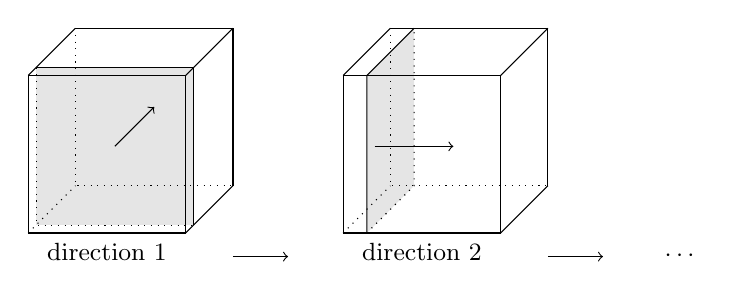
\begin{tikzpicture}
	\fill[color=gray!20] (0,0) -- (2,0) -- (2,2) -- (0,2) -- cycle;
	\draw [dotted] (0,2)  -- (0,0) -- (2,0) ;
	\draw (2,0) -- (2,2) -- (0,2) ;
	\draw (-0.1,-0.1) -- (1.9,-0.1) -- (1.9,1.9) -- (-0.1,1.9) -- cycle;
	\draw [dotted] (0.5,2.5) -- (0.5,0.5) -- (2.5,0.5);
	\draw (2.5,0.5) -- (2.5,2.5) -- (0.5,2.5);
	\draw (1.9,1.9) -- (2.5,2.5);
	\draw (-0.1,1.9)--(0.5,2.5);
	\draw (1.9,-0.1)--(2.5,0.5);
	\draw[dotted] (-0.1,-0.1)--(0.5,0.5);
	\draw[->] (1,1) -- (1.5,1.5);
	\draw(0.9,-0.1) node[below]{\small direction 1} ;
	
	\fill[color=gray!20] (4.2,-0.1) -- (4.2,1.9) -- (4.8,2.5) -- (4.8,0.5) -- cycle;
	\draw (4.2,-0.1) -- (4.2,1.9) -- (4.8,2.5);
	\draw[dotted] (4.2,-0.1) -- (4.8,0.5) -- (4.8,2.5);
	\draw (3.9,-0.1) -- (5.9,-0.1) -- (5.9,1.9) -- (3.9,1.9) -- cycle;
	\draw [dotted] (4.5,2.5) -- (4.5,0.5) -- (6.5,0.5);
	\draw (6.5,0.5) -- (6.5,2.5) -- (4.5,2.5);
	\draw (3.9,1.9) -- (4.5,2.5);
	\draw (5.9,1.9)--(6.5,2.5);
	\draw (5.9,-0.1)--(6.5,0.5);
	\draw[dotted] (3.9,-0.1)--(4.5,0.5);
	\draw[->] (4.3,1) -- (5.3,1);
	\draw(4.9,-0.1) node[below]{\small direction 2} ;
	\draw[->] (2.5,-0.4) -- (3.2,-0.4);
	\draw[->] (6.5,-0.4) -- (7.2,-0.4);
	\draw(8.2,-0.2) node[below]{\small $\cdots$} ;
	\end{tikzpicture}
	\caption{2-dimensional splitting for numerical resolution.}
	\label{fig:split2d}
\end{figure}
	
	This splitting introduces a slight approximation as the whole AFS is not updated instantaneously. When you update along the last pair of dimensions, the AFS entries have already been impacted by the changes due to the other pairs and that may induce artificial asymmetries. To minimize this numerical inaccuracy, we subdivise the time step and permute the order of the by-dimensional operator so that the first to be applied is not always the same...\\
	
	Note that in the specific case without migrations, we implemented the classical 1D-splitting, faster than the 2D one. The shape of our system (\textit{i.e} the crossed terms) is probably one of the major drawbacks of our method compared to $\partial a \partial i$ that can use 1D-splitting for every case (even with migrations).

\section{Rewriting the ugly integration loops as dot products}
	One of the consequences of the dimensional splitting is that the code becomes a bit more complex (and ugly). Especially, the integration along the different pairs of dimensions was coded through a large amount of functions involving nested loops. To make it more readable and potentially more efficient, we tried to re-arrange this part of the code replacing the loops by dot products. 
	This is pretty simple to do in the cases without migrations (1D splitting) as we just need to reshape and permute the axes using the standard python functions. Moreover it makes the code faster and more compact so we adopted this rewriting.\\
	In the general case (with migrations) it is a bit more complicated to implement as we have to write a home made reshape function that transforms the plans in vectors and then rearrange them conveniently which does not really make the code more explicit. Moreover, the only part of the code that could be impacted by this change is the dot product induced by the Crank Nicolson scheme. The system inversion, which represents here a vast majority of the computational time, is not impacted. Finally, this change does not speed up computations (it is even a bit slower in 4D) so we kept the ugly loops till we can find something better...

\section{Grid coarsening}
	A promising way to speed up the ODE system integration is to reduce the amount of ODEs! To do that, one may think about coarsening the system by not considering the equations for some entries of the AFS and interpolate them from the one we kept in the system (see Fig.\ref{fig:coarsening}). 
	 
\begin{figure}[h!]
	\centering
	\subfloat["normal" system]{\label{fig:coarse_syst}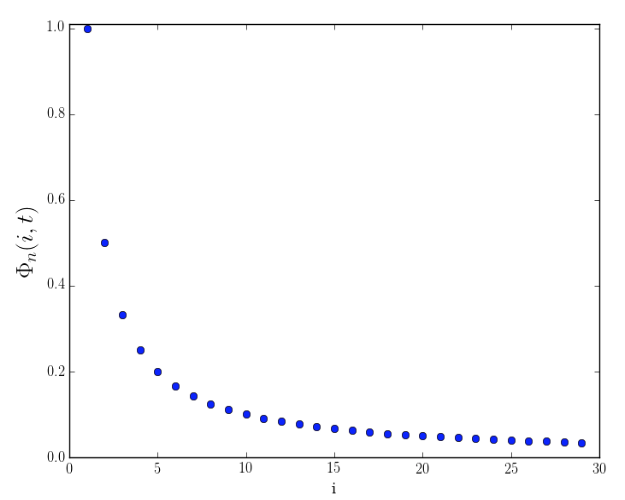
\includegraphics[scale=0.25]{figures/sfs_norm.png}} \hspace{0.2cm}               
	\subfloat[coarse system]{\label{fig:norm_syst}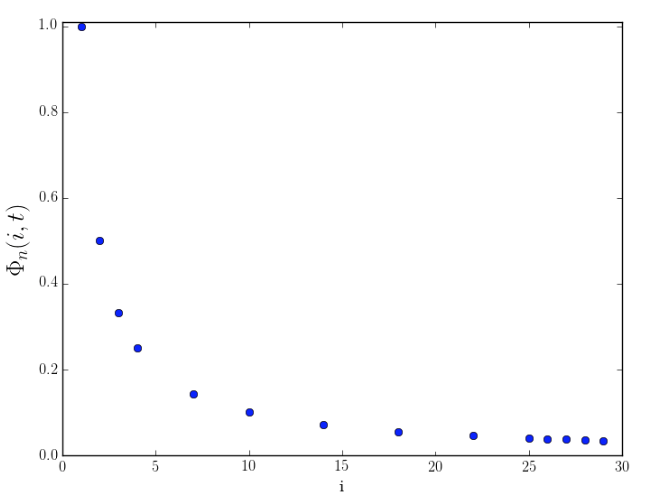
\includegraphics[scale=0.25]{figures/sfs_coarse.png}}\\
 	\caption{Example of "grid" coarsening. \ref{fig:norm_syst} represents the whole frequency spectrum. \ref{fig:coarse_syst} is the frequency spectrum in the case where we do not consider some entries.}\label{fig:coarsening}
\end{figure}

In the example provided in Figure \ref{fig:coarsening}, the "coarse" system is only composed of 16 equations \textit{versus} 31 for the classical system (counting the boundaries). So doing that, we divide by 2 the size of the system. However, the entries that we decide not to compute cannot by totally ignored as they impact the evolution of their neighbours. We have to define an interpolation function to infer these missing entries from the ones we know.
This interpolation is used twice in the process. First we compact the evolution matrix and then, after the integration, we reconstruct the entire spectrum from the coarse one. \\

One of the easiest things we can do is to use a linear interpolation: $$\Phi(i) = a\times i +b.$$
Coefficients $a$ and $b$ are computed for each missing entry using the nearest known values on the right and on the left.


-> facile a faire mais non conservatif

\section{Multi-diagonal linear solver}

\section{Adaptative time step}

\end{document}




 
